\newpage
\section{Tryout}\label{sec:tryout}

\begin{figure}[H]	% H stands for here (place right here)
	\centering
	\includegraphics[height=5cm]{figures/tryout.png}
	\caption[Optional optional]{Entscheidungsbaum}
	\label{fig:tryout}
\end{figure}

Wie auf der Abbildung \ref{fig:tryout} zu sehen ist.....


\begin{table}[H]
	\centering
	\label{tab:tryouttab}
\caption[This is an optional caption, without reference]{Local caption, with reference}
	\cite{ref:ds_1, ref:nn_1, ref:ai_1}	% Used to add cites (zitieren)

	\begin{tabular}{l c r}
		Area & Number of rooms & Price \\ \hline
		80	& 4				& 1680 \\
		100	& 5				& 2300 \\
		50	& 2.5				& 1500 \\

	\end{tabular}
\end{table}


\begin{itemize}
	\item This is an item
	\item This is another item
	\begin{itemize}
		\item This is a further item
		\item [blub] This is an item with a custom bullet point
	\end{itemize}
\end{itemize}

\begin{enumerate}
	\item This is a numbered item
	\item And so on
\end{enumerate}


\newpage
\subsection{Math examples}

Here's an example within a sentence $E =mc^2$.

And here one example $$a=v/t$$ which is centred. \\

$$-\frac{\hbar^2}{2m}\frac{d^2\Psi}{dx^2} = E\Psi$$

Fractions

$$d = v_it + \frac{1}{2} \cdot at^2$$
$$d = v_it + \sfrac{1}{2} \cdot at^2$$


Brackets:
$$\left( \frac{1}{2} \right) \cdot 2 = 1$$	% use \left( ..... \right) to match the brackets to the content
$$\left| -7 \right| = 7$$
$$\sqrt{4} = 2$$
$$\sqrt{4} \ne 1$$
$$\sqrt{4} < 5$$
$$ \pi \approx 3 $$
$$ \pi \times \sqrt{4} < 15 $$

\begin{eqnarray}	% Equation array
	3x + 14 &=& 20 \\
	3x &=& 6 \\
	x &=& 2
\end{eqnarray}

\begin{equation}
\label{eq:first}
x^2 + 3x - 7 = 0
\end{equation}

\newpage
\subsection{Graphs}




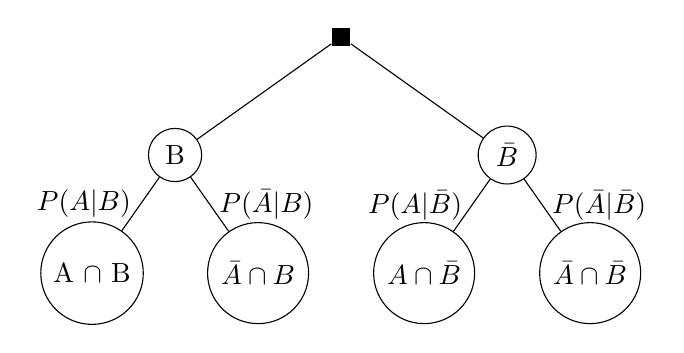
\begin{tikzpicture}[sibling distance=12em,
							%root/.style={treenode,circle,draw},
							every child node/.style={circle, draw=black},
							]
%	[align=center, sibling distance=5cm]
	\node[fill=black]{}
		child { node {B}
		[sibling distance=6em]
			child { node{A $\cap$ B}  edge from parent node[left] {$P(A|B)$} }
			child { node{$\bar{A} \cap B$} edge from parent node[right] {$P(\bar{A}|B)$}}
			}
		child{ node{$\bar{B}$}
			[sibling distance=6em]
			child{ node{$A \cap \bar{B}$} edge from parent node[left] {$P(A|\bar{B})$}}
			child{ node{$\bar{A} \cap \bar{B}$} edge from parent node[right] {$P(\bar{A}|\bar{B})$} }
		       }
	;

\end{tikzpicture}
% ****************************************************************
